%************************************************
\section{Task 1: ALF} % (fold)
\label{sec:res_alf_task}
%************************************************

%************************************************
\subsection{Question 0}
%************************************************
\emph{What level of understanding do you have at the moment about the SSM?}\\

The scale goes from 1 \emph{(Not at all)} to 7 \emph{(Expert)}.
\begin{table}[H]
	\begin{center}
		\small \begin{tabular*}{1.15\columnwidth}{lcccccr}
			\\ \hline \hline
			(1) & (2) & (3) & (4) & (5) & (6) & (7) \\ \hline \hline

		 	0 (0.0\%) & 2 (11.76\%) & 4 (23.53\%) & 4 (23.53\%) & 5 (29.41\%) & 1 (5.88\%) & 1 (5.88\%)\\ \hline
		\end{tabular*}
	\end{center}
\end{table}

\begin{figure}[H]
	\centering
	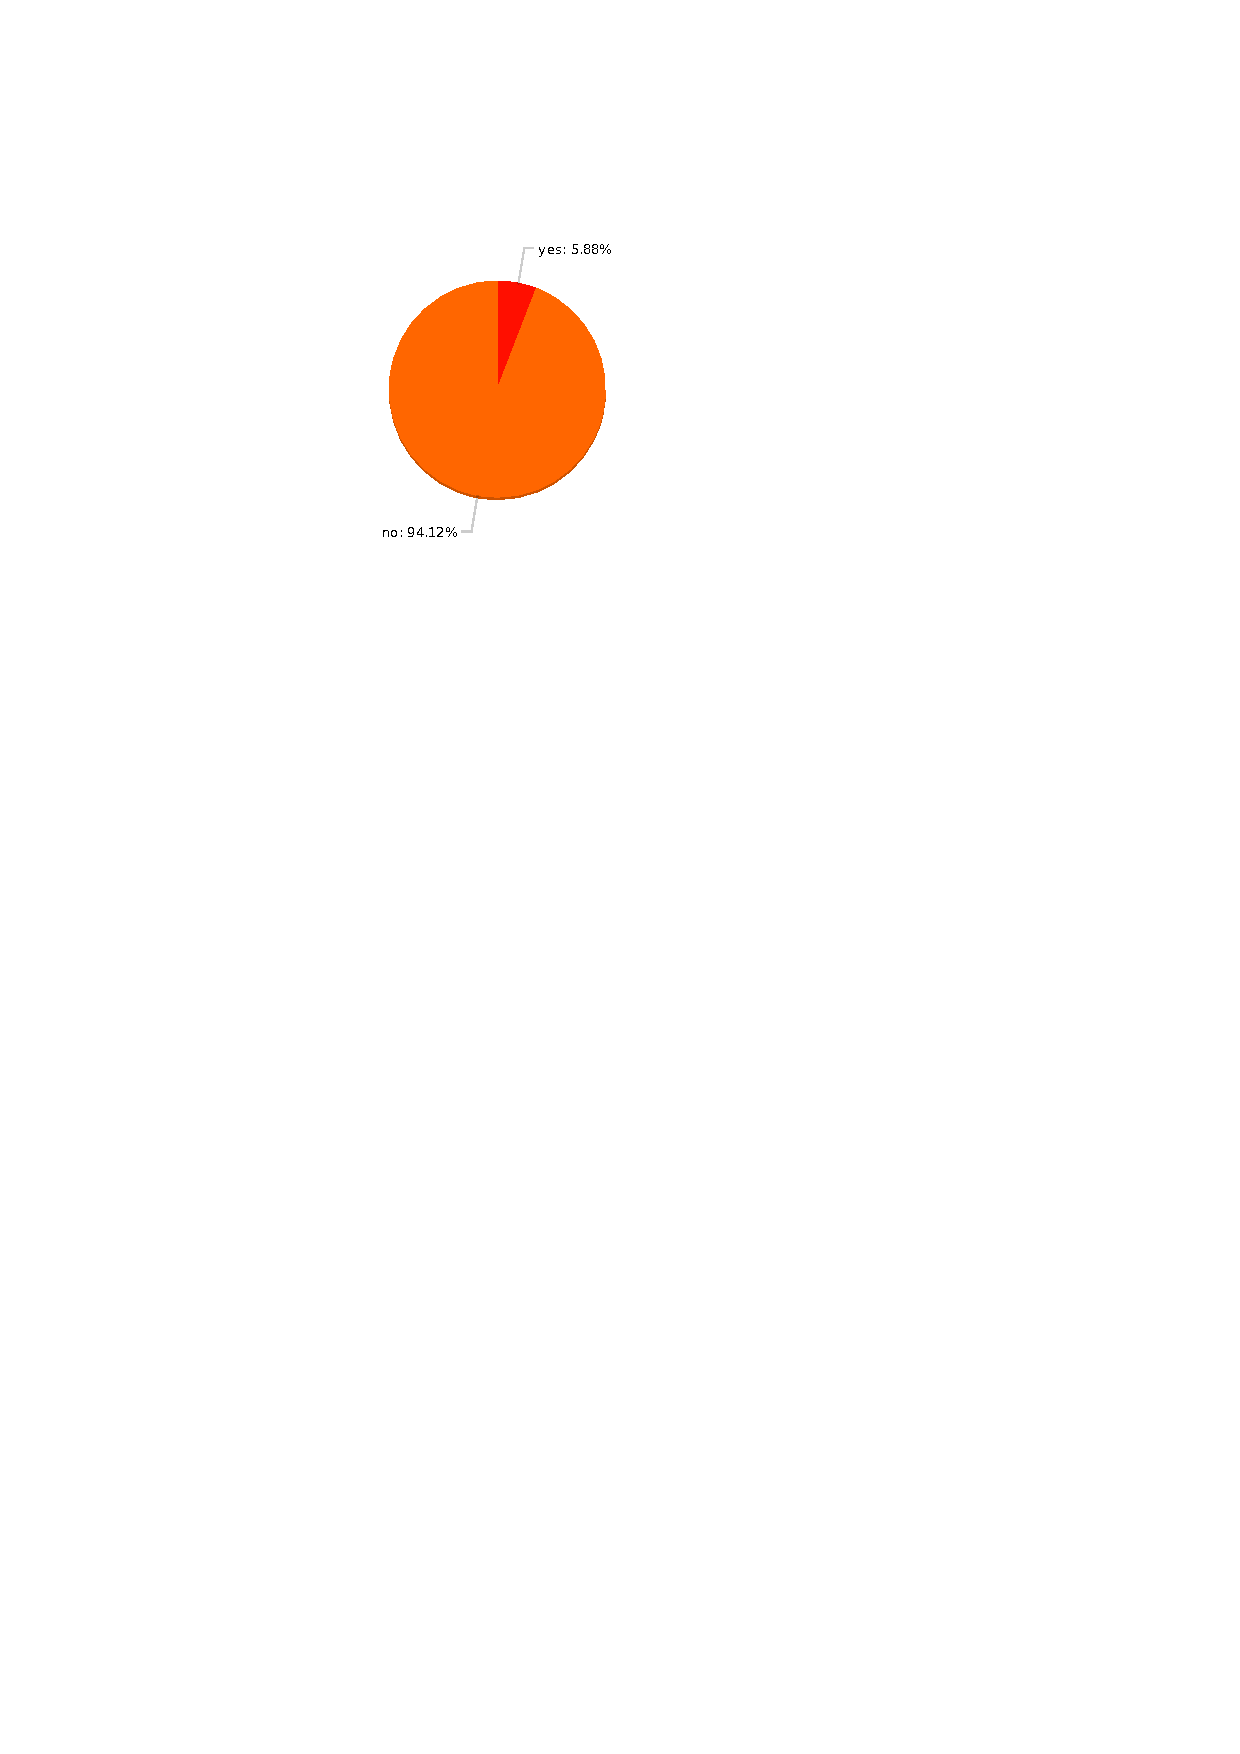
\includegraphics[width=0.6\linewidth]{gfx/Chapter_EvaluationResults/ALFTask/question0}
\end{figure}
% section sec:question0 (end)

%************************************************
\subsection{Question 1}
%************************************************
\emph{Did you find this environment a good simulation of a home?}
\begin{table}[H]
	\begin{center}
		\small \begin{tabular*}{0.35\columnwidth}{lr}
			\\ \hline \hline
			Yes & No \\ \hline \hline

		 	17 (100.0\%) & 0 (0.0\%)\\ \hline
		\end{tabular*}
	\end{center}
\end{table}
% section sec:question1 (end)

%************************************************
\subsection{Question 2}
%************************************************
\emph{How did you find the ActionDistance -- the distance from which the agent is able to interact with objects?}
\begin{table}[H]
	\begin{center}
		\small \begin{tabular*}{0.6\columnwidth}{lcr}
			\\ \hline \hline
			Too close & Close to realistic & Too far \\ \hline \hline

		 	1 (5.9\%) & 15 (88.2\%) & 1 (5.9\%)\\ \hline
		\end{tabular*}
	\end{center}
\end{table}

\begin{figure}[H]
	\centering
	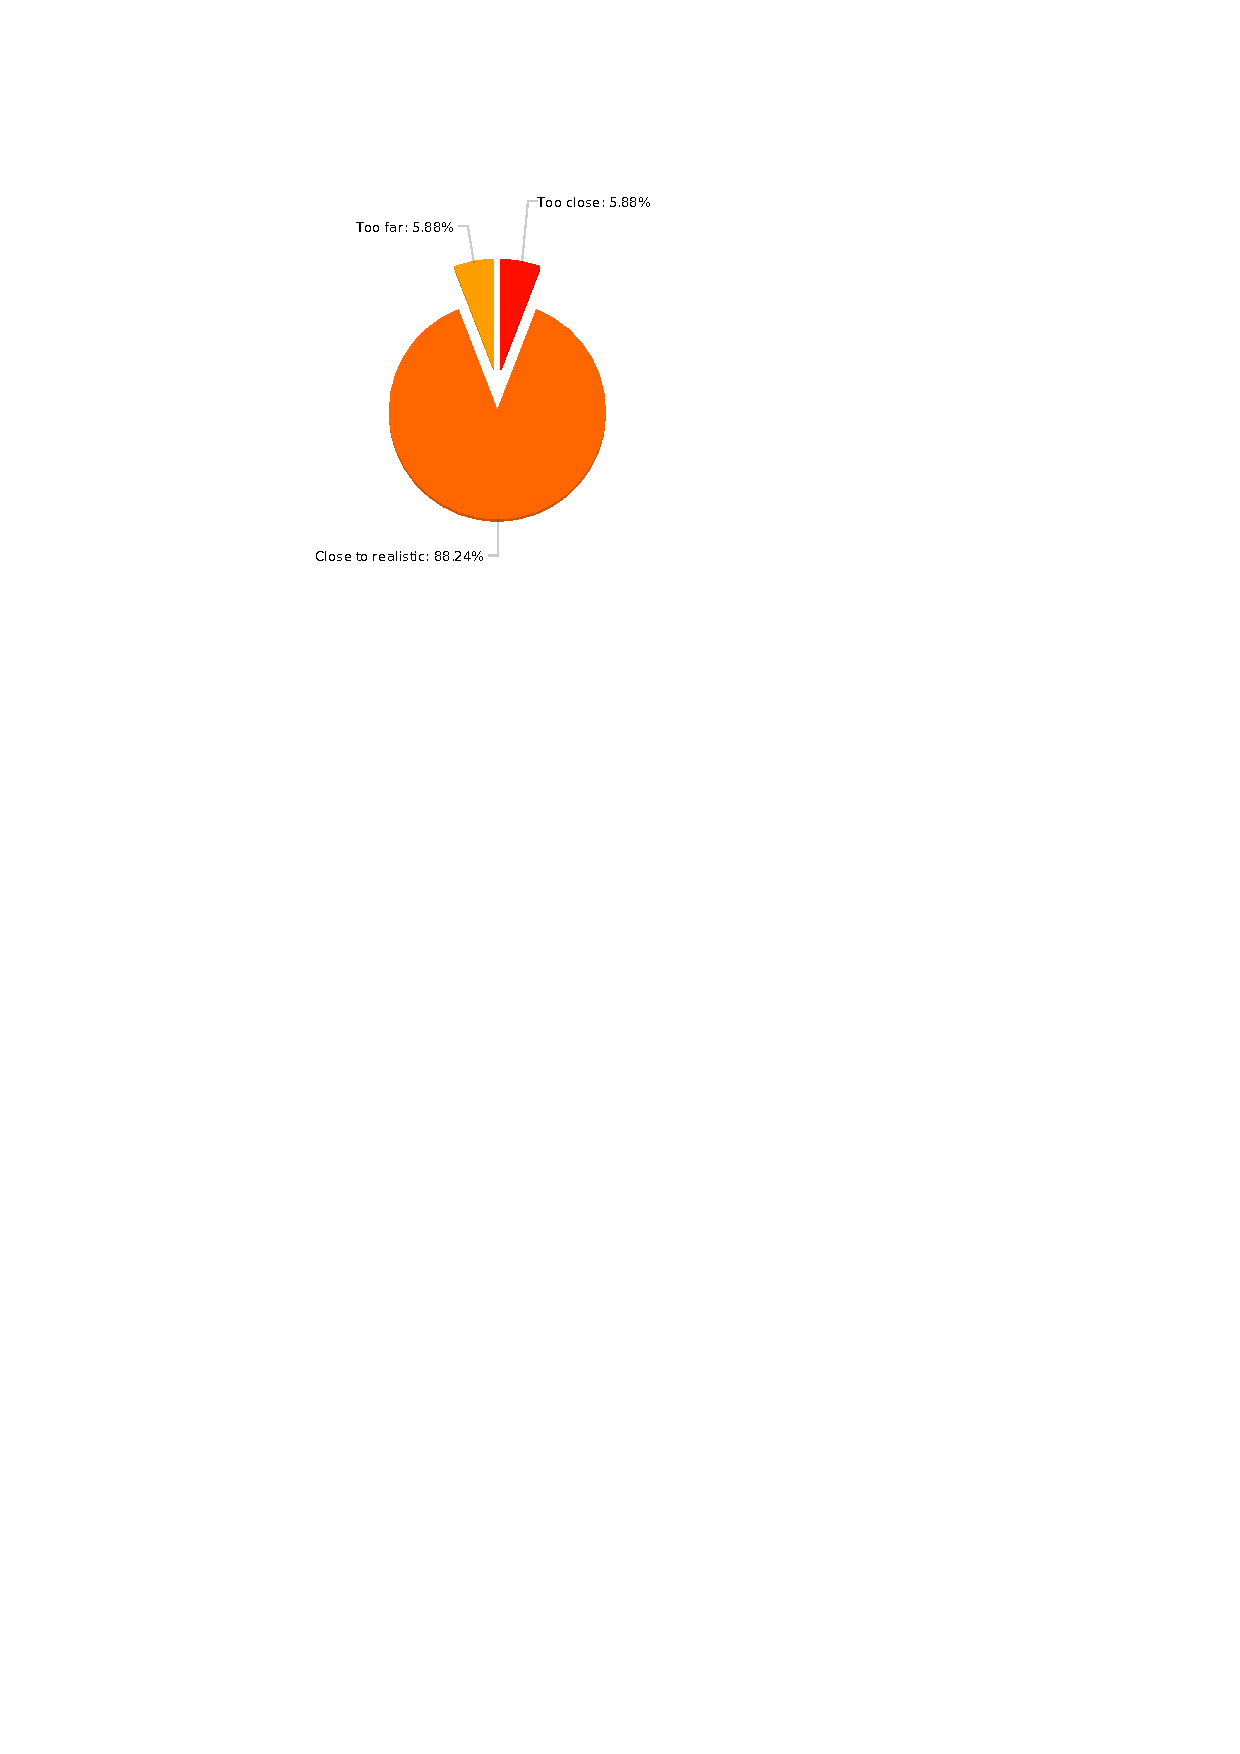
\includegraphics[width=0.6\linewidth]{gfx/Chapter_EvaluationResults/ALFTask/question2}
\end{figure}
% section sec:question2 (end)

%************************************************
\subsection{Question 3}
%************************************************
\emph{How intuitive did you find interacting with objects?}\\

The scale goes from 1 \emph{(Not intuitive at all)} to 7 \emph{(Highly intuitive)}.
\begin{table}[H]
	\begin{center}
		\small \begin{tabular*}{1.15\columnwidth}{lcccccr}
			\\ \hline \hline
			(1) & (2) & (3) & (4) & (5) & (6) & (7) \\ \hline \hline

		 	0 (0.0\%) & 0 (0.0\%) & 2 (11.76\%) & 2 (11.76\%) &	4 (23.53\%) & 2 (11.76\%) & 7 (41.18\%)\\ \hline
		\end{tabular*}
	\end{center}
\end{table}

\begin{figure}[H]
	\centering
	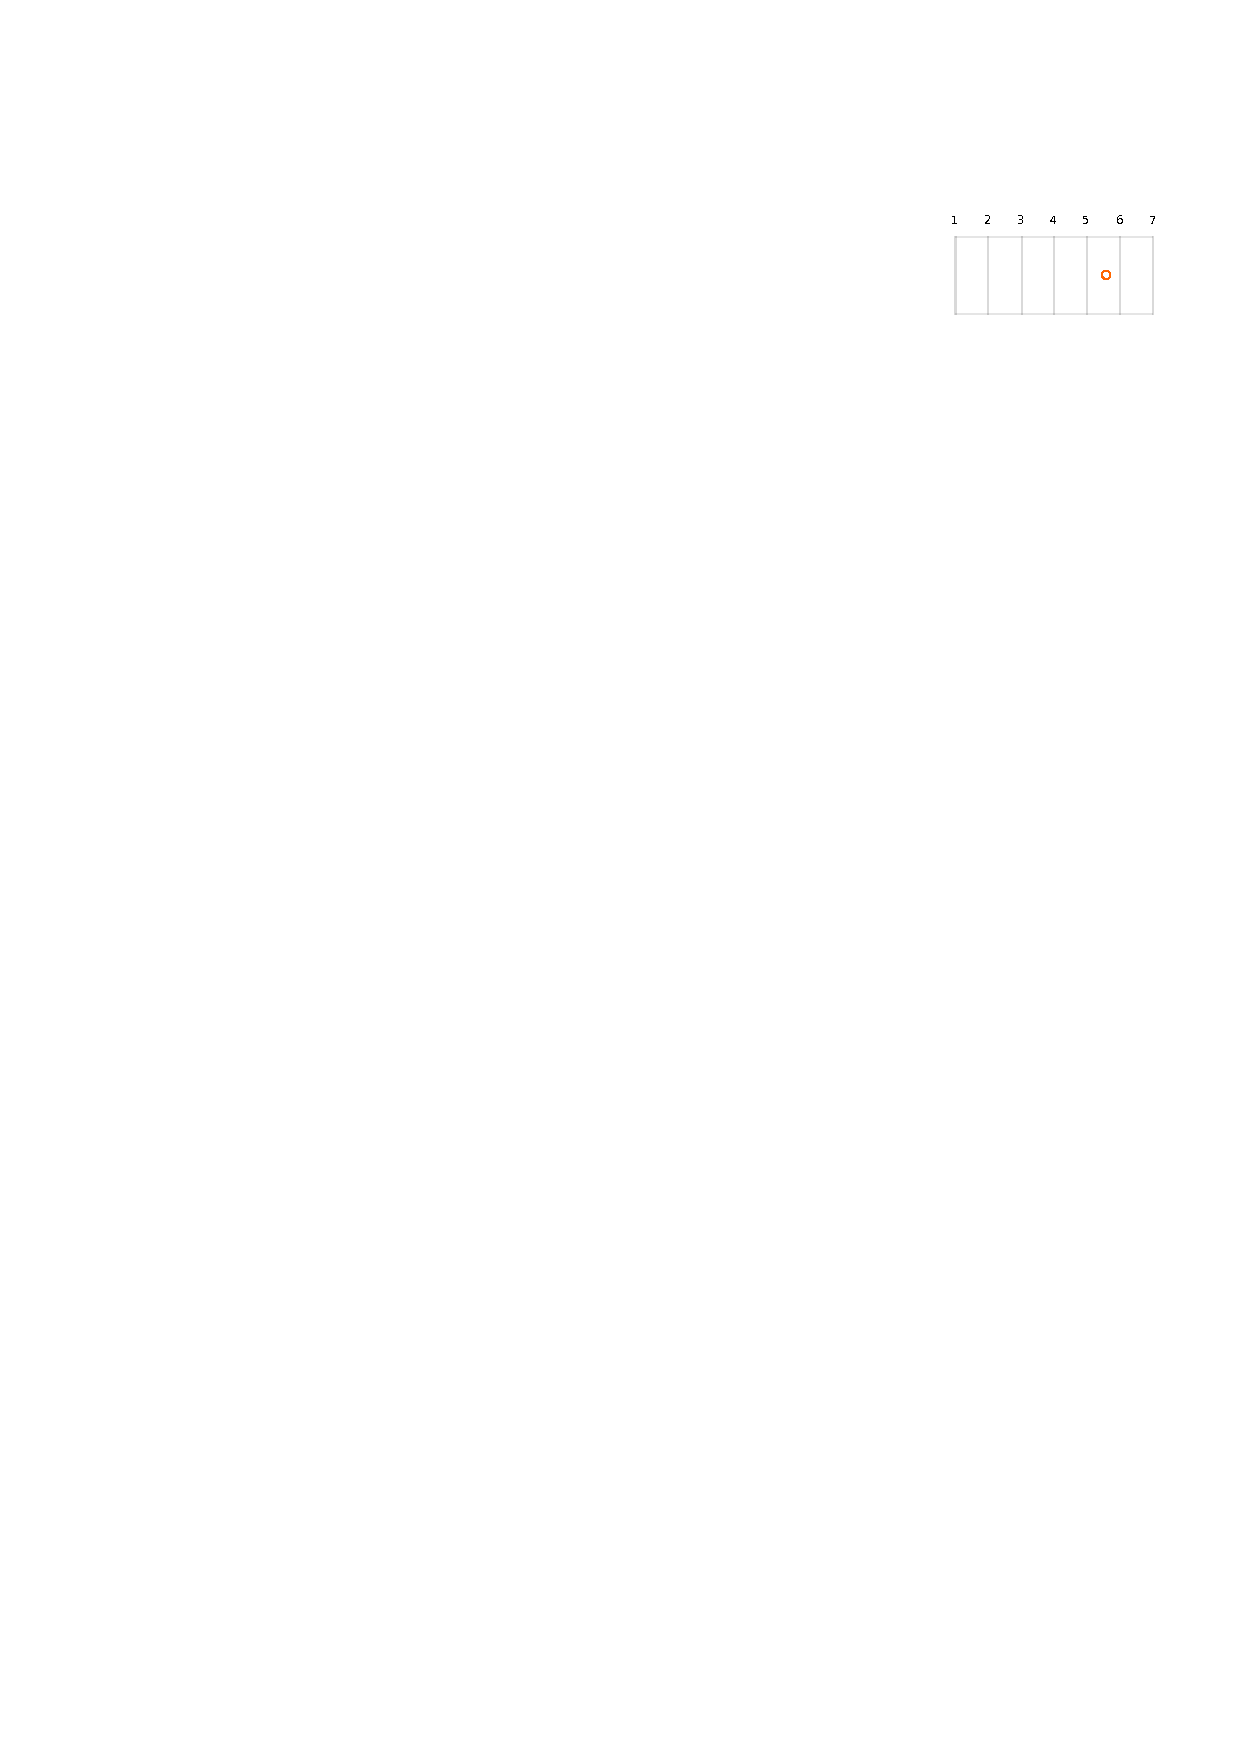
\includegraphics[width=0.6\linewidth]{gfx/Chapter_EvaluationResults/ALFTask/question3}
\end{figure}
% section sec:question3 (end)

%************************************************
\subsection{Question 4}
%************************************************
\emph{Were all the objects correctly classified in the perception space?}
\begin{table}[H]
	\begin{center}
		\small \begin{tabular*}{0.35\columnwidth}{lr}
			\\ \hline \hline
			Yes & No \\ \hline \hline

		 	10 (58.8\%) & 7 (41.2\%)\\ \hline
		\end{tabular*}
	\end{center}
\end{table}

\begin{figure}[H]
	\centering
	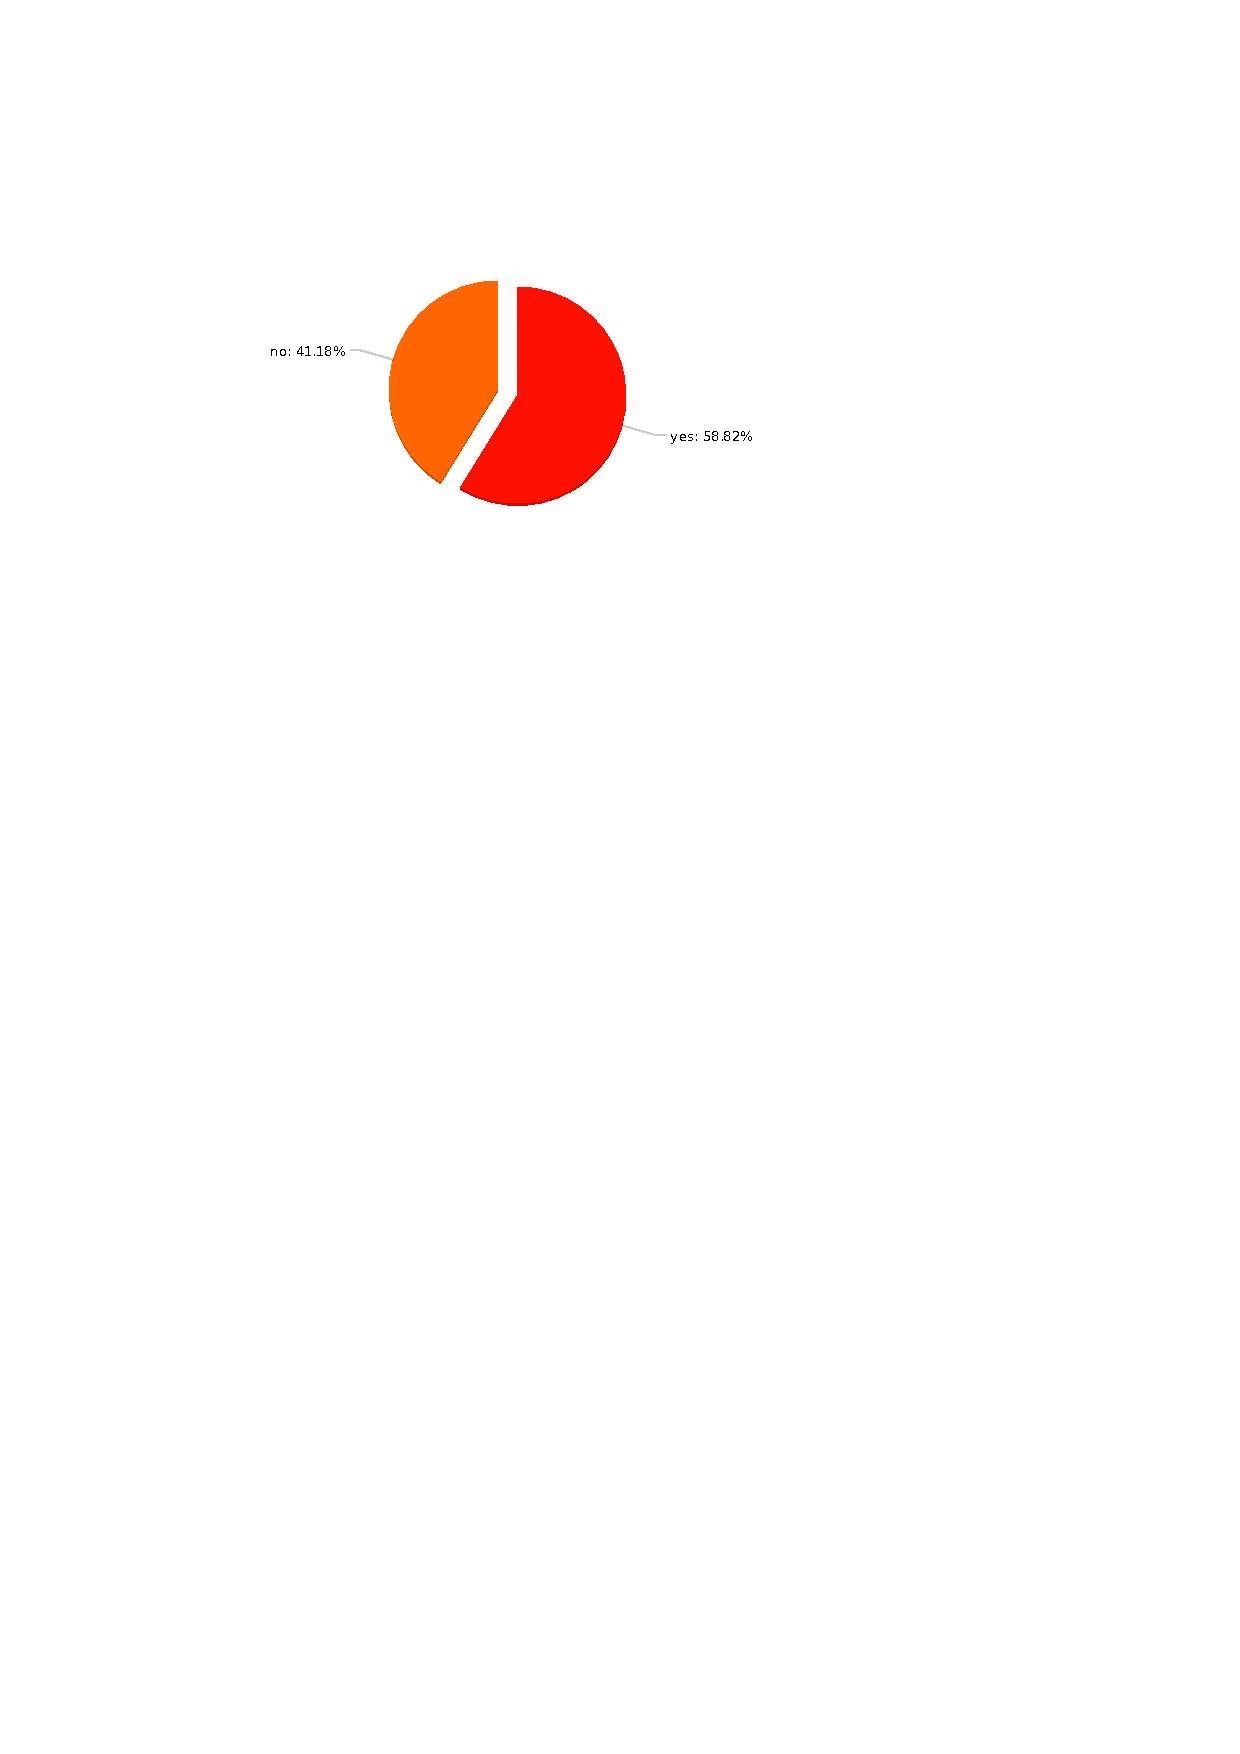
\includegraphics[width=0.6\linewidth]{gfx/Chapter_EvaluationResults/ALFTask/question4}
\end{figure}

\emph{If No, describe at least one in which one or more objects were not correctly classified}
\begin{itemize}
	\item If I am in the corner of the kitchen facing the bedroom I can see the corner of the closet but it does not appear in any other space apart from the world space. And I can use the mouse to try and interact with it and it says ''Closet, you are too far!'' so maybe it should have appeared in the perception space at least.
	\item The living room table while standing in the bedroom. It could ''see'' the cup and the laptop, but not the table.
	\item Standing behind the couch, it only identified the laptop, not the closet, even though it was visible. If I moved a little back, it identified the closet too.
	\item the action space is sometimes too determined by where the cursor cross is, and not whether the object is in front of you or not. e.g., placing the cursor just on the side of the laptop makes the laptop be outside the action space. moving the cursor over the laptop makes the laptop enter the action space. the laptop should be in the action space also when the cursor is just beside it.
	\item I was standing in the kitchen door. The laptop and cup were in the perceptive space although they were kind of hidden by the sofa and the TV although more visible was not.
	\item The table and chairs in the kitchen -- they are not classified in the perception space.
	\item There were objects in the apartment which were not classified at all: toilet, window, chairs... 
	\item When standing next to the piano I think the TV should have been in the perception space.

\end{itemize}
% section sec:question4 (end)

%************************************************
\subsection{Question 5}
%************************************************
\emph{Was the ContextClient displaying the updated context information of the system fast enough to reflect the surroundings of the agent?}
\begin{table}[H]
	\begin{center}
		\small \begin{tabular*}{0.35\columnwidth}{lr}
			\\ \hline \hline
			Yes & No \\ \hline \hline

		 	13 (76.5\%) & 4 (23.5\%)\\ \hline
		\end{tabular*}
	\end{center}
\end{table}

\begin{figure}[H]
	\centering
	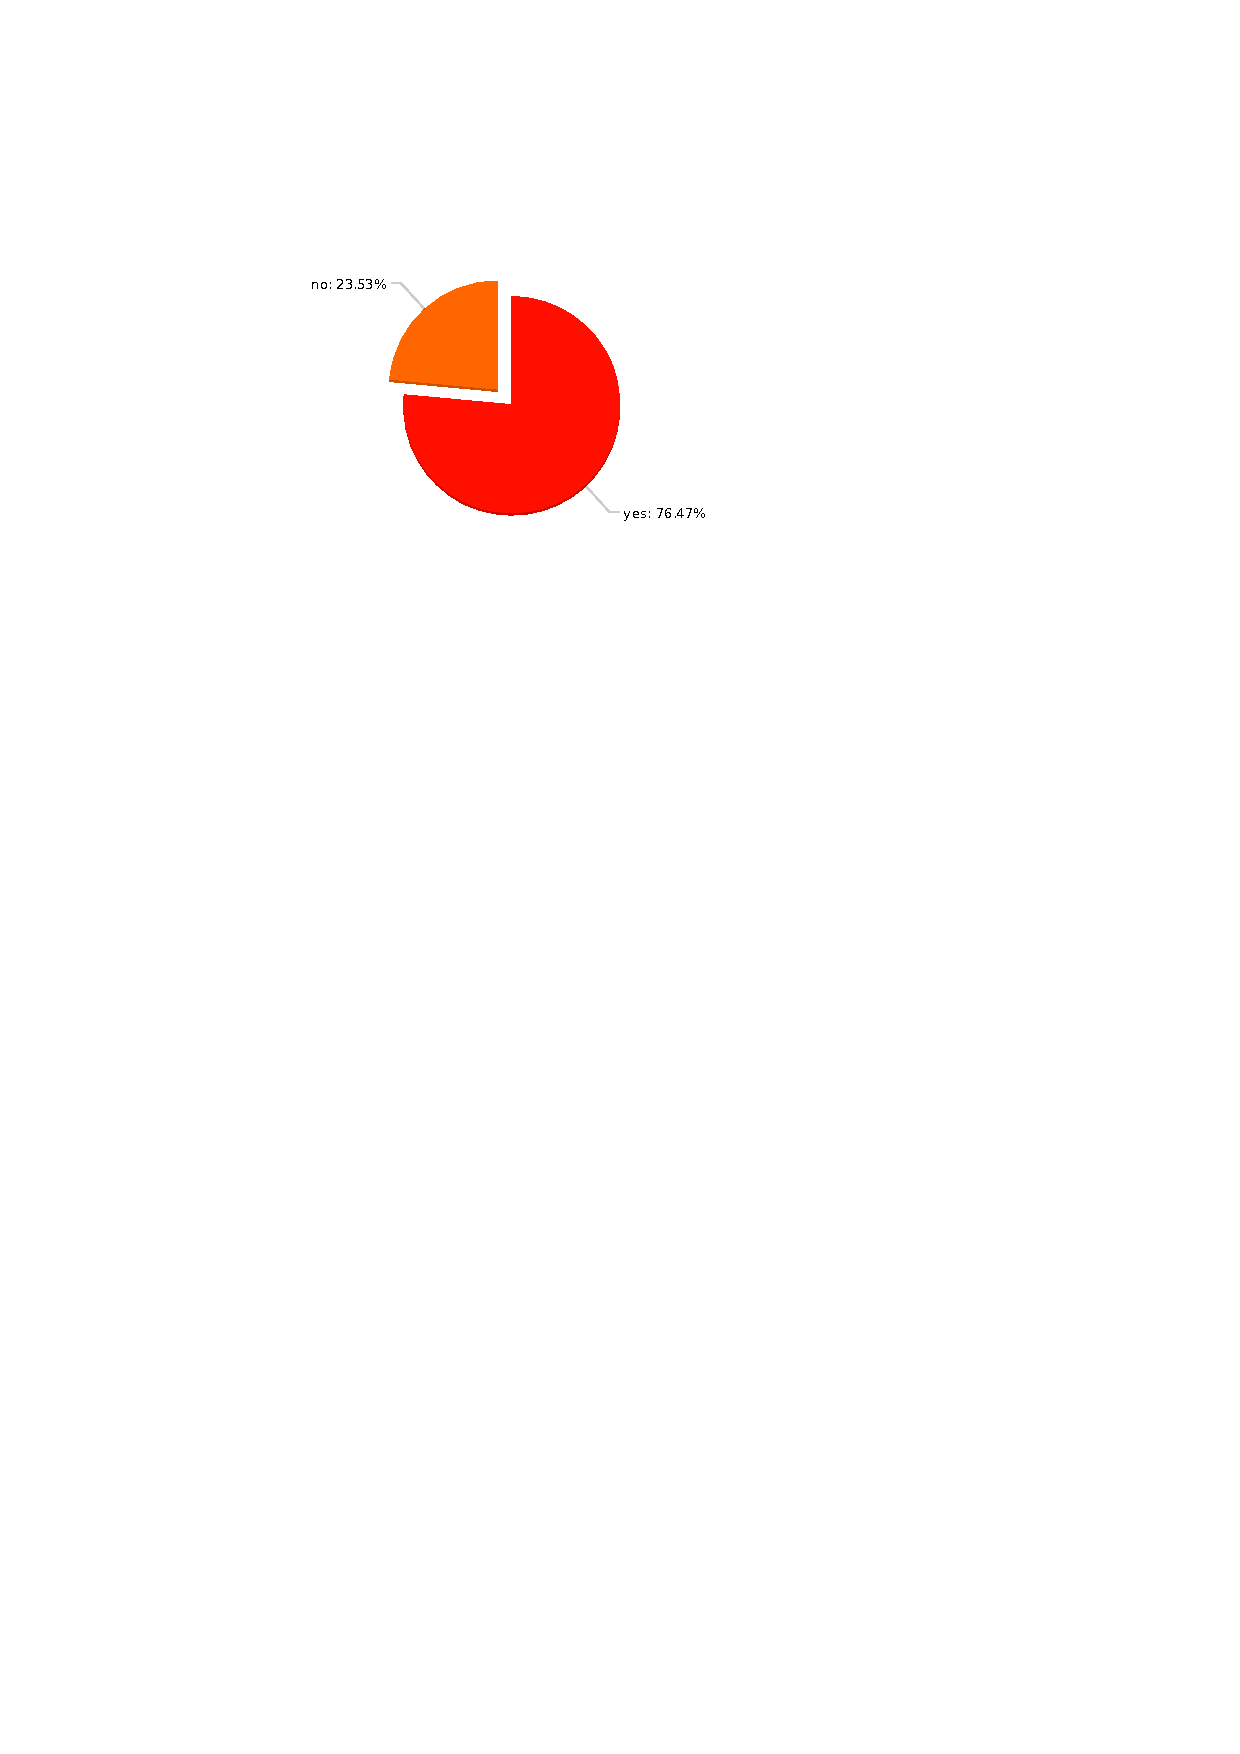
\includegraphics[width=0.6\linewidth]{gfx/Chapter_EvaluationResults/ALFTask/question5}
\end{figure}

\emph{If No, why?}
\begin{itemize}
	\item The ContextClient update rate was decent for the ADL service but might require some improvement for other applications.
	\item A tricky situation would be objects suddenly appearing in the perception space and being used shortly thereafter. For example, a phone may ring behind the user and the user instinctively turns and picks it up (use). This example would be solved if the perception space is not limited to the visual stimulus, however it illustrates some exceptions that might cause the low update rate to be a problem.
\end{itemize}
% section sec:question5 (end)

%************************************************
\subsection{Question 6}
%************************************************
\emph{Do you think the SSM would be the right model for the ADL Service?}
\begin{table}[H]
	\begin{center}
		\small \begin{tabular*}{0.35\columnwidth}{lr}
			\\ \hline \hline
			Yes & No \\ \hline \hline

		 	17 (100.0\%) & 0 (0.0\%)\\ \hline
		\end{tabular*}
	\end{center}
\end{table}
% section sec:question6 (end)

%************************************************
\subsection{Question 7}
%************************************************
\emph{Do you find this simulation useful over implementing the system directly into a real system?}
\begin{table}[H]
	\begin{center}
		\small \begin{tabular*}{0.35\columnwidth}{lr}
			\\ \hline \hline
			Yes & No \\ \hline \hline

		 	17 (100.0\%) & 0 (0.0\%)\\ \hline
		\end{tabular*}
	\end{center}
\end{table}

\emph{Why?}
\begin{itemize}
	\item The simulation could provide a cost effective way of gaining valuable insight into the design of an Assisted Living Facility before such a facility is constructed. The location of various object around the room and distance between them could be determined using this simulation so as to maximize the efficiency of an ADL Service
	\item Simulations are always good for better understanding of the real systems. 
	\item In this particularly case, a simulation is a must. A every day life has a lot of interactions, and some are necessary (taking pills), and other are harmful (forgetting the stove turned on).
	\item I think it is very useful especially for testing the implementation of a ADL Service or other similar services for other environments. It is not needed to implement the real system to know how the service works if you can simulate it, one can detect bugs and malfunctions in the system before implementing it in a real environment. It is also cost effective.
	\item Because it offers a controllable environment to test the concepts and calibrate the initial assumptions of how the system should be designed before creating the actual devices.
	\item Because of the cost. You can implement it basically for free. Afterwards, you can use the simulation to do a cost estimate of the implementation into a real system.
	\item I think such a system must be validated before being deployed to ensure the safety of the people involved. Also, I think it would be a lot more cost-effective as it would help in discovering faults early on, before something is implemented (therefore significantly cheaper to correct)
	\item Give you a perception of how people interact with the objects.
	\item Lower costs in case of trial and error.
	\item Helps in the real implementation, like finding the best location for sensors.
	\item Faster feedback loop.
	\item A simulation is a reliable and cheap proof of concept for me.
	\item It allows the discovery of corner cases. 
	\item As most simulations, it helps in better understanding of the system.
	\item Same reasons as the ones highlighted in the ''Introduction'' section.
\end{itemize}
% section sec:question7 (end)

%************************************************
\subsection{Question 8}
%************************************************
\emph{Did the simulation run smoothly?}
\begin{table}[H]
	\begin{center}
		\small \begin{tabular*}{0.35\columnwidth}{lr}
			\\ \hline \hline
			Yes & No \\ \hline \hline

		 	15 (88.2\%) & 2 (11.8\%)\\ \hline
		\end{tabular*}
	\end{center}
\end{table}

\begin{figure}[H]
	\centering
	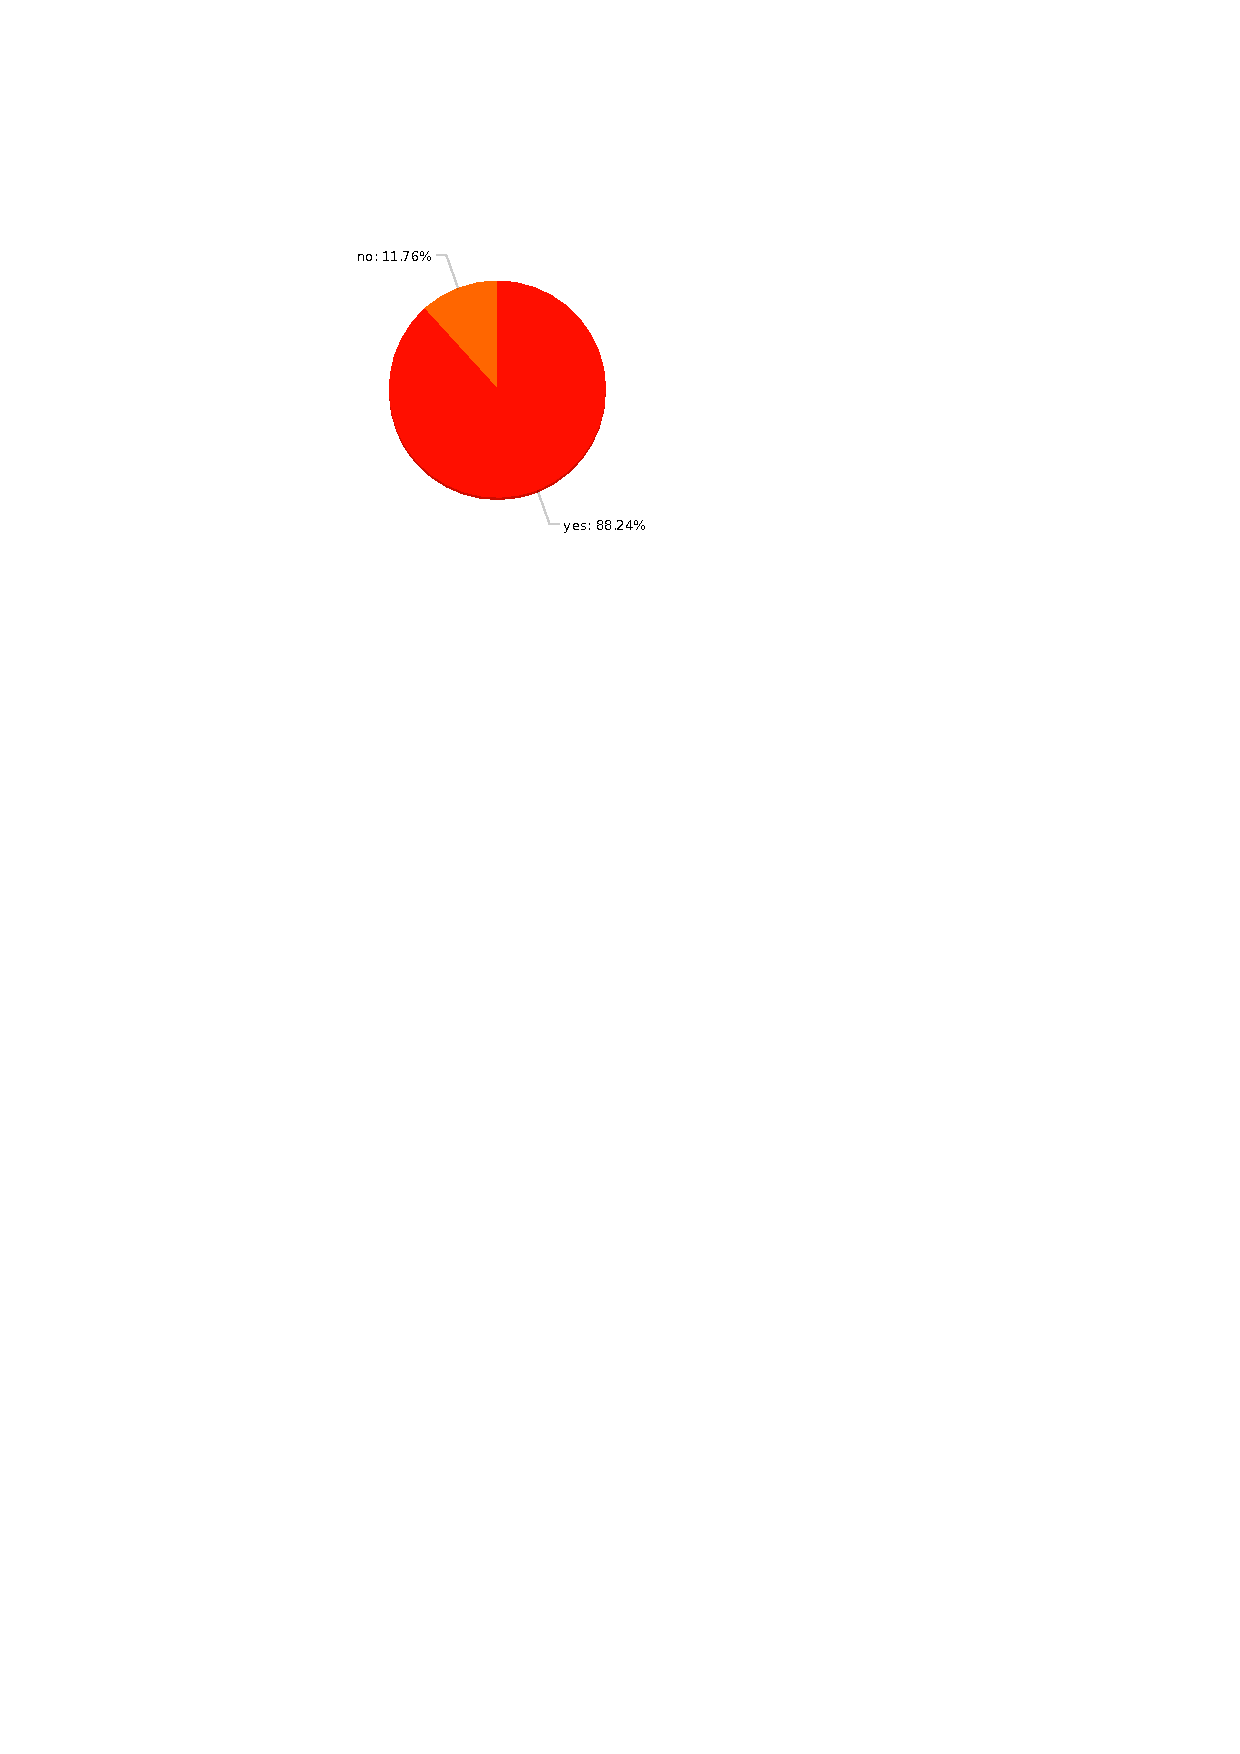
\includegraphics[width=0.6\linewidth]{gfx/Chapter_EvaluationResults/ALFTask/question8}
\end{figure}

\emph{If No, describe a situation it did no perform well.}
\begin{itemize}
	\item There was a glitch when I couldn't move forward when getting out of bed. I had to move in a different direction and after that come back and approach the closet.
	\item the simulation window run on the external screen was placed in the middle of the screen as default and could not be moved. in order to save screen space (enable to have the task description on the side for instance) it would be good to be able to move the simulation window around.
\end{itemize}
% section sec:question8 (end)

%************************************************
\subsection{Question 9}
%************************************************
\emph{Please leave in this last field any feedback that comes to your mind! (ideas for improvements, bugs you might have found, things that you liked, etc)}

\begin{itemize}
	\item It was not clear to me if the elements in the action space are influenced only by the proximity of the agent to them or also by what elements are in the selected space. The reason I am thinking of this is because I can imagine objects which should be only handled if the agent is currently holding another object. For example, the ADL service could generate a warning when the agent tries to handle a dangerous object (like a hot plate) without having some protecting item in the selected space like some gloves (this is not a very good example but you get the idea :) )
	\item One more thing I thought about was taking into memory of the agent for the recognizable space. I assume in time, the dynamics of the recognizable space change and objects which at the beginning are only in perception space, once they have moved into the recognizable space, they will stay there as the agent can remember them and their position.
	\item Nice playing with the application :).
	\item I could not use the MyGame.app and had to run it from jMonkeyPlatform (system info: MOAC OSX, version 10.7.4).
	\item I think moving around was very close to reality and I liked the fact that it was aware of the obstacles. For example, you could not just move forward through the couch to get to the coffee table.
	\item The Piano playing actions were nice.
	\item integrate with a Virtual Reality kit
	\item create a MMO EgoSim app where users (not just programmers) can create their own environments => you get feedback on a larger scale, see what other kinds of problems could be solved using the egocentric paradigm
	\item I really like the interaction, but what it was not quite clear to me was what is the ''Last distance from agent'' useful for. Some of the objects displayed there were not even in the perception space and still they had a distance. It did not know what I was supposed to do with the info or how to check it. Maybe a ''Current distance from the agent'' would be more useful?
	\item there seems to be a discrepancy between how the action space is modelled when you drop an object vs. when you pick up an object: dropping an object on another object is possible from afar, but picking it up isn't. Example: while standing in front of the sink, holding the coffee pot, I could drop the coffee put to the left of the sink but then not pick it up directly afterwards because it was regarded to be too far away. picking and dropping should demand the same distances, or?
	\item You can pick up the stove
	\item When you put the coffee pot down, it looks like it's in the stove not above it
	\item The refresh is not very accurate, the application runs smooth, good interaction.
	\item I liked the interaction with the piano
	\item I like the idea, but I would not implement it in a home where the elderly lives on its own. I think the ADL Service is more suitable for a retiring home where there is also human personnel which can intervene in exceptional cases.
	\item Change the cursor to reflect when an object is in the ActionSpace.
	\item I consider the condition for an object to enter the perception space to be too weak. A user cannot identify an object if only a ''pixel'' is within his field of vision. Humans are built to recognize patterns, therefore a pattern-oriented metric could be used.
	\item For instance, the introduction of a diversity factor would help the simulation. If enough ''diversity'' of the object is within the perception space, it could trigger its presence in the perception space.
	\item Given the high system requirements I would have expected a better graphics/game engine.
\end{itemize}
% section sec:question9 (end)

% section sec:res_alf_task (end)